\section{Experiments}
\label{sec:intro}

We conducted three different experiments where we evaluated the accuracy of the models in terms of how many test commands were exactly translated
into corresponding test actions. 
\citet{Lake:Baroni:2017} found that RNNs models are achieve nearly perfect performance when tested on a random split of SCAN but accuracy drops significantly
(down to around 20\% for their best performing model) when the network is tested on composing new meanings after being exposed only to shorter samples.

In order to make our results comparable with previous work on SCAN each training set consists of 100,000 examples sampled with replacement
from each related train/test split. We decided to replicate experiment 1 of \cite{Lake:Baroni:2017} that simply uses a random split
of the SCAN dataset divided into a train (80\%) and test (20\%) set. This would act as a first comparison with the RNNs results reported in their work.

\subsection{Experiment 1: random split and primitive generalization}
\label{subsec:exp1}

After a preliminary experiment we found a subset of parameters showing reasonable performance and conduceted a large hyperparameters
search on every split.
We varied batch sizes (in term of number of tokens in the batch: 25, 50, 100, 200, 500 and 100), learning rates
0.1, 0.01, 0.001), the embedding dimensions (128, 256, 512), amount of dropout used (0, 0.25, 0.5) \cite{srivastava:eta:2014}, number of convolutional
layers for both the encoder and decoder (6, 7, 8, 9, 10) and width of the convolutional kernel (3, 4, 5).
We then cross validated the top-300 models across 5 different runs. Accuracy and standard deviation are presented in figure \ref{fig:exp1}. 
We inspected the average accuracy of the model note that the amount of standard deviation of the top-300 models reached a performance range with a lower limit that was always
considerably lower than the best model for each split, making us think that considering the top-300 models was
a right choice that included tha real best model for every split. In other words, the accuracy for the best model and the 300th one formed a large range.
\footnote{This might not seem the case for the results on the random split where the range is (95.17, 99.97). However the standard deviation across all 300 models does not
exceed 2.7}
When analyzing the the resulting models for every split we computed a \textbf{best overall model} across all splits which
was a model trained with a learning rate of 0.01, a 25 tokens per batch, dropout applied with probability 0.25, it had 6 layers in both the encoder and the decoder,
embedding dimension of 512, a convolutional kernel of width 5. Such model was ranked 13th on the random split (with an accuracy of 99.92\% off by 0.05\%), 
32th on the jump split (60.67\% accuracy, off by 8.62\% compared to the top performing model for the split),
and 2nd in the template split (53.25\% accuracy, off by 3.45\%)
Experiment 2 and 3 in section \ref{subsec:exp2} and \ref{subsec:exp3} used the aforementioned model.

\begin{figure}[h]
    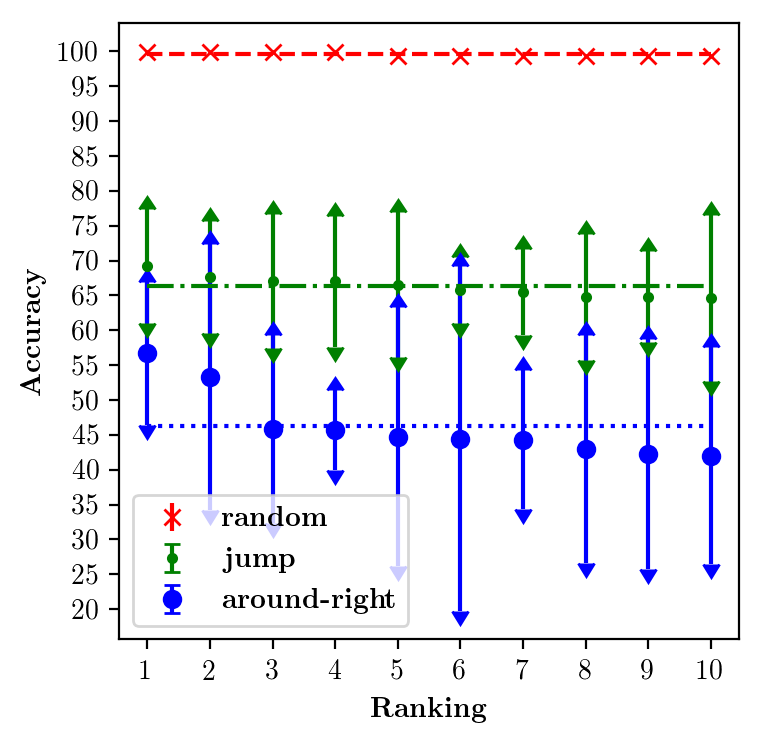
\includegraphics[width=.5\textwidth,keepaspectratio]{figures/accuracies_all_splits.png}
    \centering
    \caption{Accuracies for the top-10 models on every split. Dashed lines report split means}
    \label{fig:exp1}
\end{figure}


% 219.08612pt
% 3.0314
\subsection{Experiment 2: second-order modifiers and kernel study}
\label{subsec:exp2}

\iffalse

\begin{figure}[h]
    \centering
    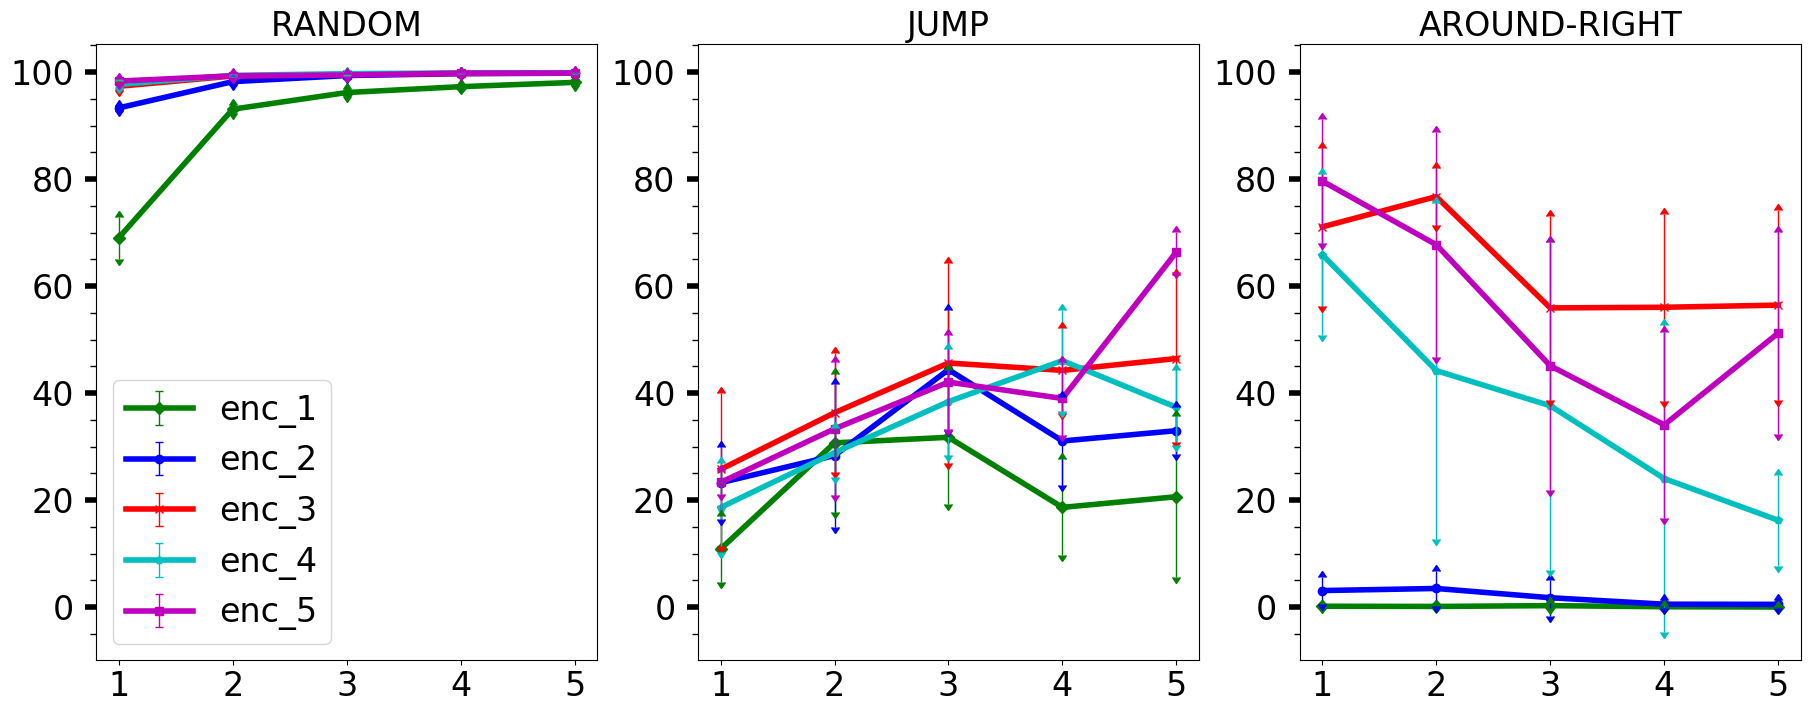
\includegraphics[width=.5\textwidth,keepaspectratio]{figures/kernel_exp.png}
    \caption{Accuracy for kernel experiment}
    \label{fig:kernel_exp}
\end{figure}

\fi


\begin{figure*}[h]
    \centering
    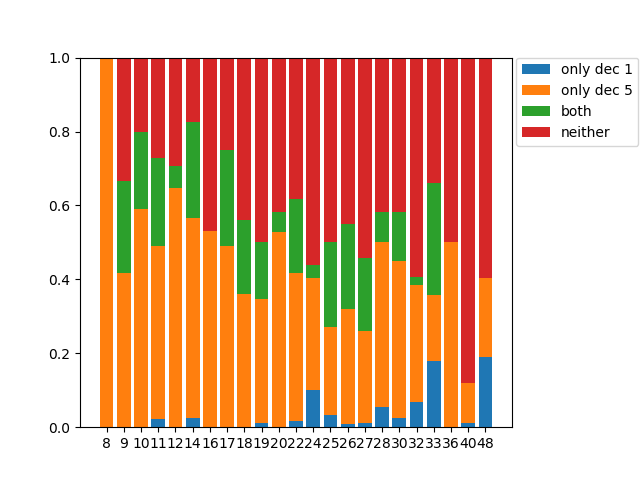
\includegraphics[width=.4\textwidth,keepaspectratio]{figures/jump_subset_out.png}
    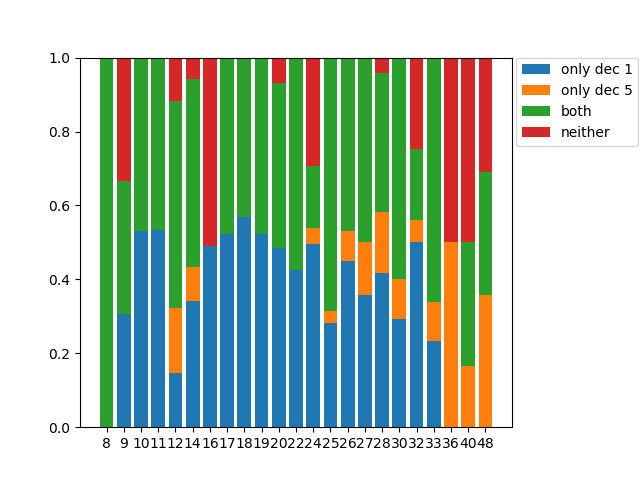
\includegraphics[width=.4\textwidth,keepaspectratio]{figures/template_subset_out.png}
    \caption{Performance distribution for jump and template splits with 5- and 1-decoder widths.}
    \label{fig:kernel_width}
\end{figure*}


\ldots For the random split, we observe the expected pattern in which
both wider encoder and decoder windows lead to perfect
performance. The jump results are less clear-cut, but respect the same
trend: the narrowest encoder-decoder combination achieves the worst
performance, and the widest one the top one. For the around-right
split, it's also better to have the widest encoder, but now we find
that top performance is achieved with the \emph{narrowest} decoder
(width$=$1). Since the novel output sequences in this split are by
construction long, we would have rather expected that models that keep
track of larger window in decoding would have fared better. To gain
some insight on this behaviour, we looked at the performance
distribution across outputs of different (ground-truth) lengths in the
two experiments. Keeping encoder width fixed at 1,
Fig.~\ref{fig:kernel_width} reports the proportions of cases that were
correctly handled only with decoder width 1, 5, with either or
neither. The figure is based on items cases occurring in both data
sets, but the same pattern is confirmed when looking at the whole
generalization sets. We see more cases where both widths worked in
around-right, as expected as we have already established this as an
easier challenge for our CNNs. In general, though, we find that the
wide-decoder jump model behaves quite similarly to the narrow-decoder
around-right model, getting most of its gain from shorter
sequences. One interesting difference is that for around-right we
observe an inversion in performance for the longer sequences, where
actually the wider decoder outperforms the narrower one, in accordance
with our intuition that more context should help longer execution
tasks. Looking qualitatively at the errors, we note that, for both
splits, the narrower decoder needs to skip chunks of commands (e.g.,
executing ``jump around right'' with 3 instead of 4 right turns
followed by jump), whereas the wider kernel seems more likely to
replace commands (e.g., turning left instead of right) than
undershooting the length. Quantitatively, this is supported by the
fact that, for both splits, the narrow kernel errors have considerably
larger variance with respect to ground-truth length. While these
observations confirm the observation that a wider decoder kernel helps
with length management, we still have no insight on why the shorter
kernel should be better on the around-right split. Future work should
pursue a better understanding of how kernel widths affect linguistic
processing in CNNs.



\subsection{Experiment 3: ablation study on attention}
\label{subsec:exp3}

Due to the importance of the attention mechanism for our convolutional architecture we decided to conduct study with the best-overall model
and the attention only on specific layers. Results are presented in \ref{fig:exp3}...

\begin{figure}[h]
    \centering
    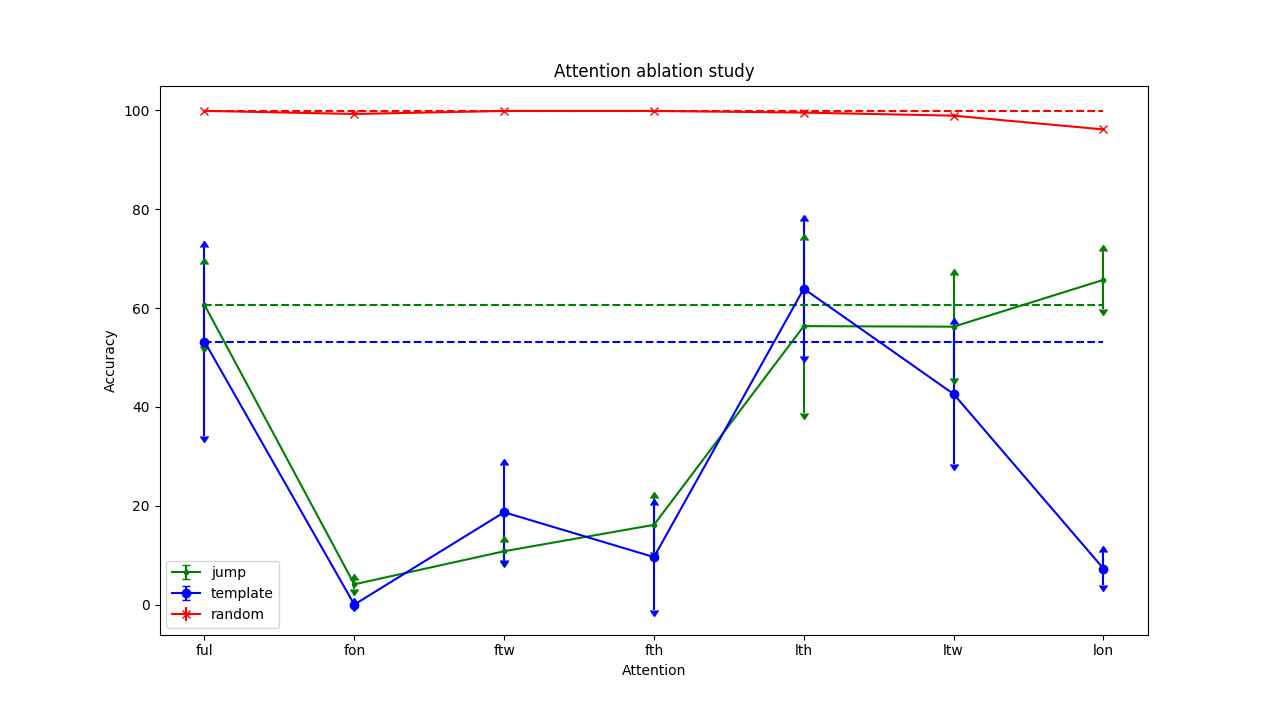
\includegraphics[width=.5\textwidth,keepaspectratio]{figures/attention_exp.png}
    \caption{Accuracy for attention experiment}
    \label{fig:exp3}
\end{figure}

